%!TEX program = xelatex
\documentclass[a4paper, UTF8]{ctexrep}
\usepackage{ctex}
\usepackage{amsmath}
\usepackage{multirow}
\usepackage{amssymb}
\usepackage{graphicx}
\usepackage{geometry}
\usepackage{bm}
\usepackage{subfigure}
\usepackage{float}
\usepackage{array}
\usepackage{makecell}

\renewcommand\thesection{\arabic{section}}

\begin{document}
	\begin{titlepage}
		\centering
		\vspace{6cm}
		\LARGE{\textbf{Computer Vision HW1}}\\
		\vspace{4cm}
		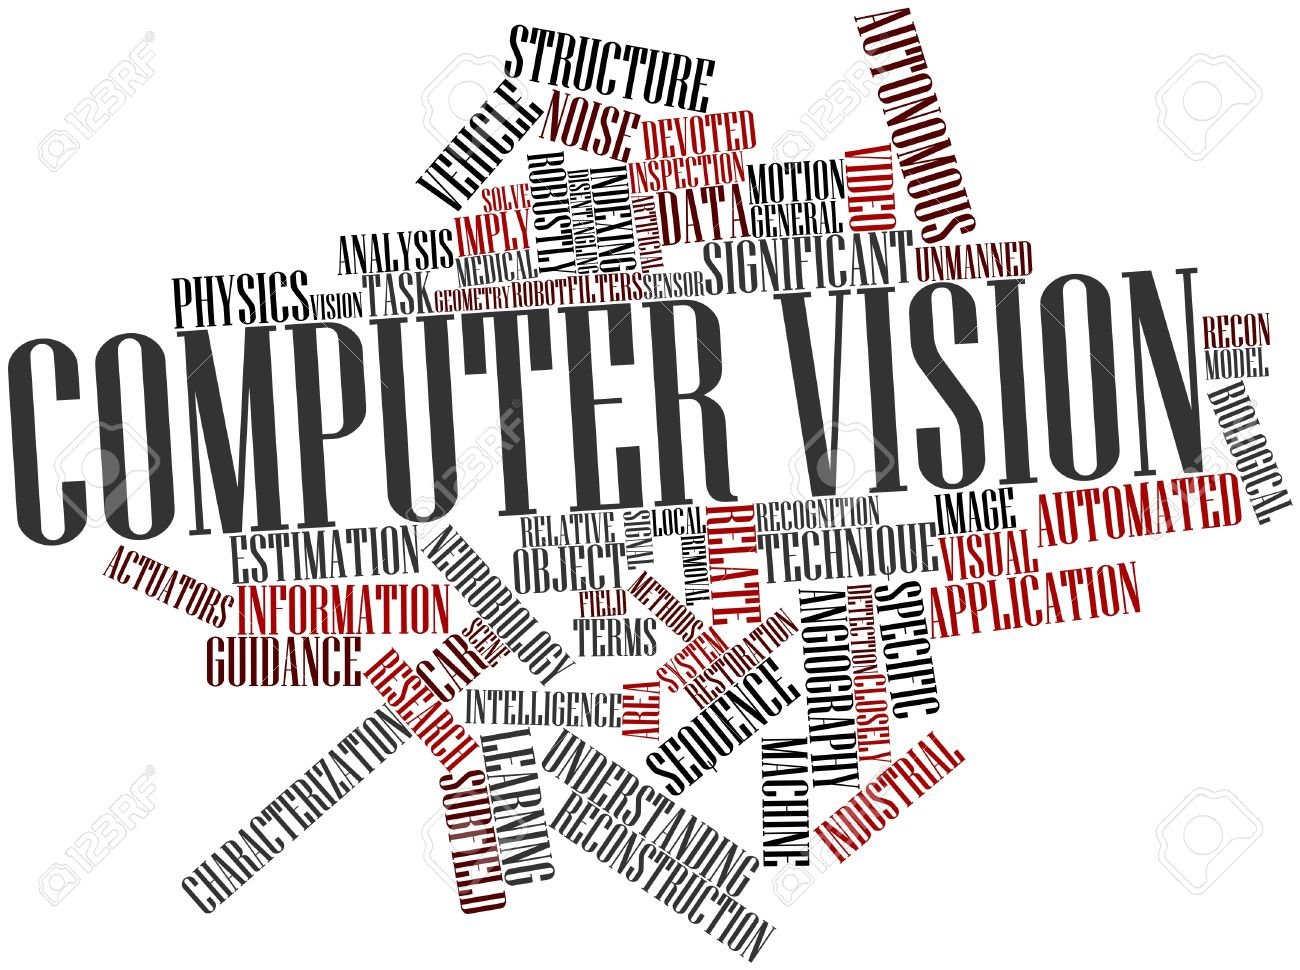
\includegraphics[width=0.8\textwidth]{cv.jpg}\\
		\vspace{5cm}
		\normalsize{安捷 1601210097}\\
		\normalsize{\today}
	\end{titlepage}
  \section{算法实现介绍}
    在这一次作业中,我按照作业要求,分别实现了Harris角点检测算法与SIFT特征检测与描述子生成算法,并针对作业中要求的具体问题,基于MATLAB编程实现了相关要求,其中,Harris角点检测算法我使用了MATLAB自带Harris角点检测函数;SIFT算子我使用了vl-feat工具包。
  \section{脚本功能介绍}
    为完成作业要求,我共编写三个MATLAB脚本,下面分别介绍其功能及对应的问题:
    \begin{description}
      \item[harris\_robustness\_test.m] 对应于作业的问题1,用于测试harris角点检测算法对于旋转、缩放的鲁棒性;
      \item[sift\_robustness\_test.m] 对应于作业的问题2,用于测试SIFT检测子对于图像旋转、缩放的鲁棒性;
      \item[sift\_descriptor\_robustness\_test.m] 对应于作业的问题3,用于测试SIFT描述子对于图像亮度、对比度、噪声、模糊的鲁棒性;
    \end{description}
  \section{各脚本参数设置}
    \subsection{harris\_robustness\_test.m参数设置}
      \begin{table}[htbp!]
        \centering
        \begin{tabular}{ccc}
        \hline
        参数名称 & 参数值 & 参数含义 \\
        \hline
        IMG\_PATH & 'cover\_1.jpg' & 图像路径 \\
        MIN\_QUALITY & 0.01 & Harris角点检测阈值 \\
        ROTATE\_ANGLE & 15 & 旋转角度 \\
        SCALE\_FACTOR & 1.2 & 缩放倍数 \\
        \hline
        \end{tabular}
        \caption{harris\_robustness\_test.m参数表}
      \end{table}

    \subsection{sift\_robustness\_test.m参数设置}
    \clearpage
      \begin{table}[htbp!]
        \centering
        \begin{tabular}{ccc}
        \hline
        参数名称 & 参数值 & 参数含义 \\
        \hline
        IMG\_PATH & 'cover\_1.jpg' & 图像路径 \\
        PEAK\_THRESH & 1 & SIFT算法峰阈值 \\
        EDGE\_THRESH & 5 & SIFT算法边阈值 \\
        ROTATE\_ANGLE & 15 & 旋转角度 \\
        SCALE\_FACTOR & 1.2 & 缩放倍数 \\
        \hline
        \end{tabular}
        \caption{sift\_robustness\_test.m参数表}
      \end{table}

    \subsection{sift\_descriptor\_robustness\_test.m参数设置}
      \begin{table}[htbp!]
        \centering
        \begin{tabular}{ccc}
        \hline
        参数名称 & 参数值 & 参数含义 \\
        \hline
        IMG\_PATH & 'building.jpg' & 图像路径 \\
        PEAK\_THRESH & 1 & SIFT算法峰阈值 \\
        EDGE\_THRESH & 5 & SIFT算法边阈值 \\
        ROTATE\_ANGLE & 15 & 旋转角度 \\
        SCALE\_FACTOR & 1.2 & 缩放倍数 \\
        BRIGHTNESS\_MINUS\_MAX & -100 & 最大亮度减小值 \\
        BRIGHTNESS\_PLUS\_MAX & 100 & 最大亮度增加值 \\
        BRIGHTNESS\_CHANGE\_LEVEL & 20 & 亮度增减幅度 \\
        CONTRAST\_MIN & 0.5 & 最小对比度调整值 \\
        CONTRAST\_MAX & 2.0 & 最大对比度调整值 \\
        CONTRAST\_CHANGE\_LEVEL & 0.25 & 对比度调整幅度 \\
        NOISE\_MIN & 0 & 最小高斯噪声标准差 \\
        NOISE\_MAX & 30 & 最大高斯噪声标准差 \\
        NOISE\_CHANGE\_LEVEL & 5 & 高斯噪声标准差调整幅度 \\
        GAUSS\_MIN & 1 & 最小高斯模糊标准差 \\
        GAUSS\_MAX & 10 & 最大高斯模糊标准差 \\
        GAUSS\_CHANGE\_LEVEL & 1 & 高斯模糊标准差调整幅度 \\
        \hline
        \end{tabular}
        \caption{sift\_descriptor\_robustness\_test.m参数表}
      \end{table}

	\section{运行结果及作业问题解答}
		鉴于在上一节已经详细列出了我在实现算法的过程中使用的参数,因此,在这里我不再详细叙述算法实现中的参数,只是在回答作业中问题的时候给出必要的参数,并且,我将主要以图表的方式来展示结果。
		\subsection{Robustness of Harris Keypoints to Rotation and Scaling}
			\subsubsection{(a)}
				这里我设置的参数MIN\_QUALITY= $0.01$,针对cover\_1.jpg,检测到了516个角点,结果如下:
				\begin{figure}[htbp!]
					\centering
					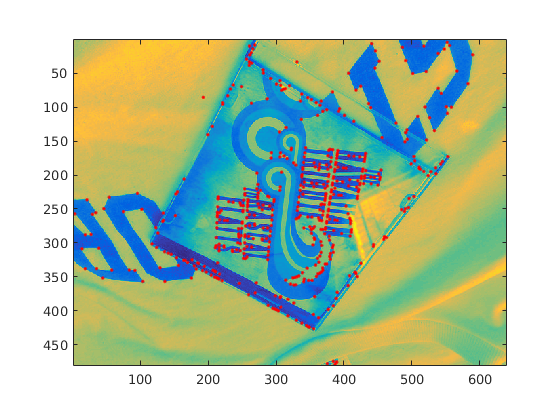
\includegraphics[width=0.8\textwidth]{hw1_fig1.png}
					\caption{Harris角点检测的结果}
				\end{figure}
				从上图中可以看出,角点主要位于中间英文字母的边缘部分及证件的边缘部分,为了研究主要角点所在的位置,我绘制了已检测出角点权重的分布图,如下:
				\clearpage
				\begin{figure}[htbp!]
					\centering
					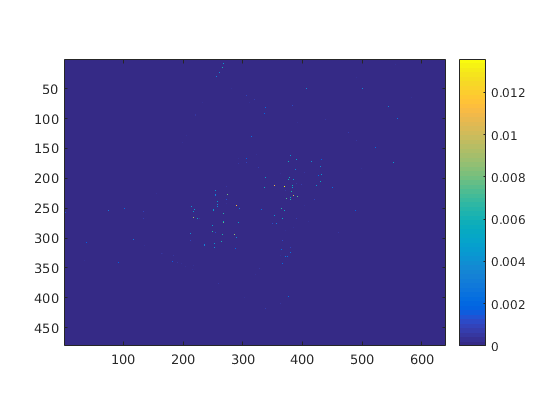
\includegraphics[width=0.8\textwidth]{hw1_fig2.png}
					\caption{Harris角点的权重}
				\end{figure}
				从图中可以看出,主要亮点均位于证件中字母所在的位置,这一结果证实了我上述断言,即:角点主要位于字母的边缘及证件的边缘部分。
			\clearpage
			\subsubsection{(b)}
				\begin{figure}[htbp!]
					\centering
					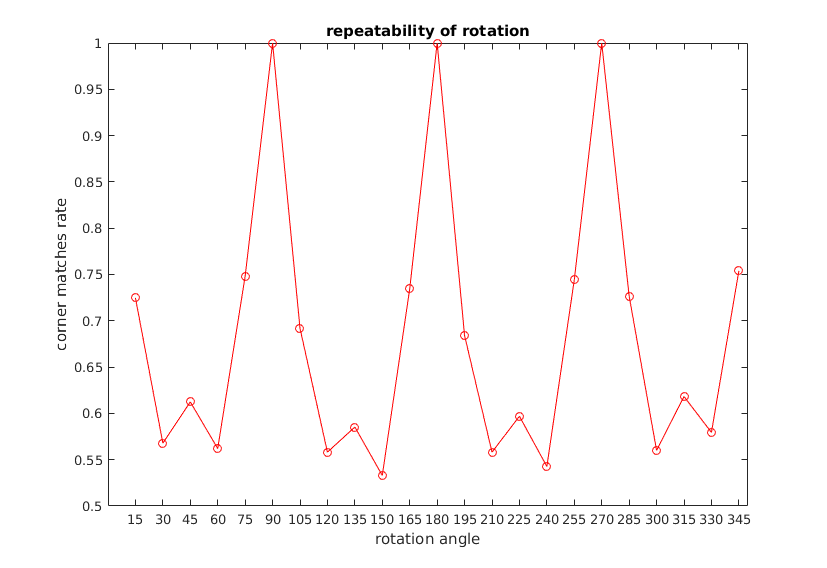
\includegraphics[width=0.8\textwidth]{hw1_fig3.png}
					\caption{图像旋转情况下Harris角点检出率的分布}
				\end{figure}
				从图中可以看出,图像旋转时,在旋转角度为0,90,180,270,360度时,Harris角点的检出率为100\%,而其他角度Harris角点的检出率也有明显的对应特点,产生这种情况的原因在于Harris角点检测中采用的差分格式,由于Harris算子使用的离散差分不具有旋转对称性,且图像旋转非上述角度时存在插值问题,因此Harris算子很难找到对应的角点,导致了检出率较低。
			\clearpage
			\subsubsection{(c)}
				\begin{figure}[htbp!]
					\centering
					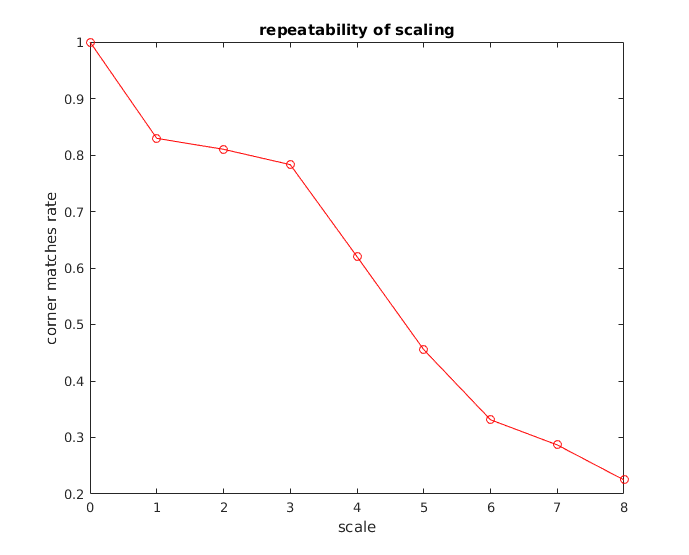
\includegraphics[width=0.8\textwidth]{hw1_fig4.png}
					\caption{图像缩放情况下Harris角点检出率的分布}
				\end{figure}
				从图中可以看出,Harris在缩放的情况下不具有较好的鲁棒性。
			\clearpage
			\subsubsection{其余数据的数值实验结果}
				\begin{figure}[htbp!]
					\centering
					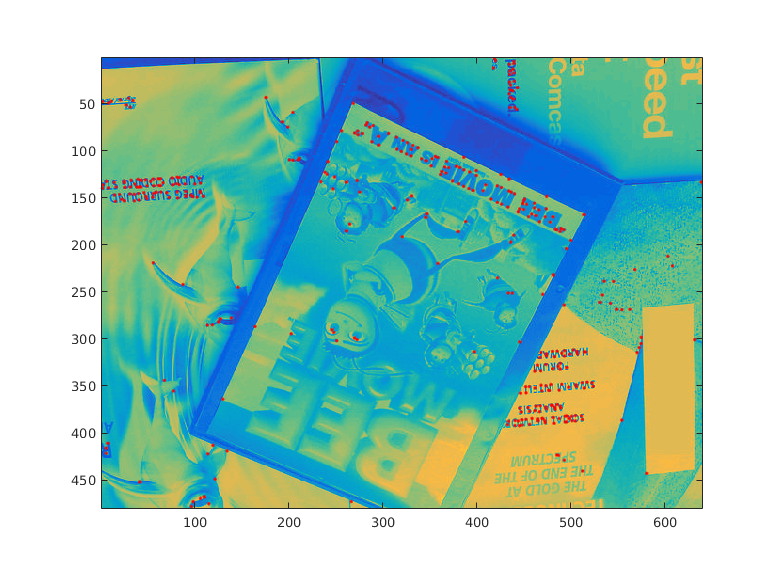
\includegraphics[width=0.8\textwidth]{hw1_fig5.png}
					\caption{Harris角点检测的结果}
				\end{figure}
				\clearpage
				\begin{figure}[htbp!]
					\centering
					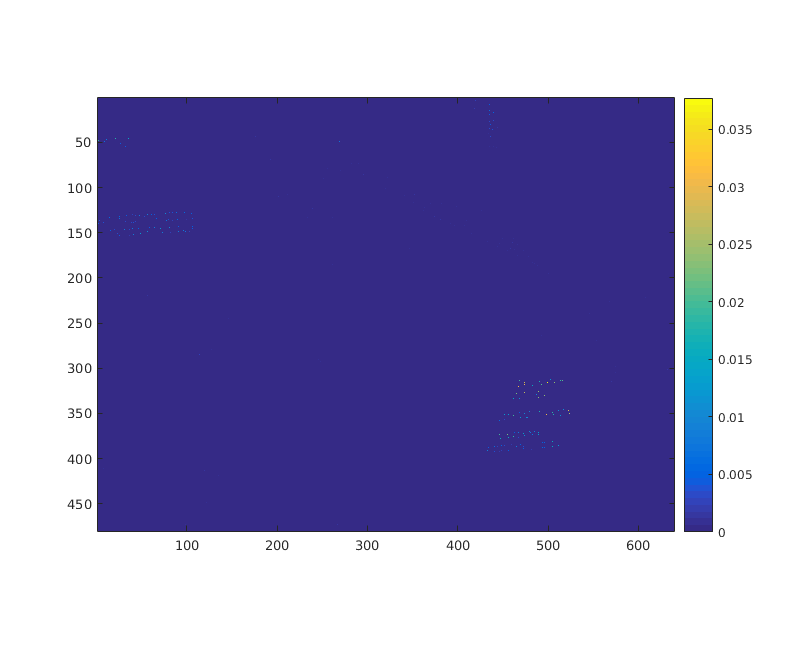
\includegraphics[width=0.8\textwidth]{hw1_fig6.png}
					\caption{Harris角点的权重}
				\end{figure}
				\clearpage
				\begin{figure}[htbp!]
					\centering
					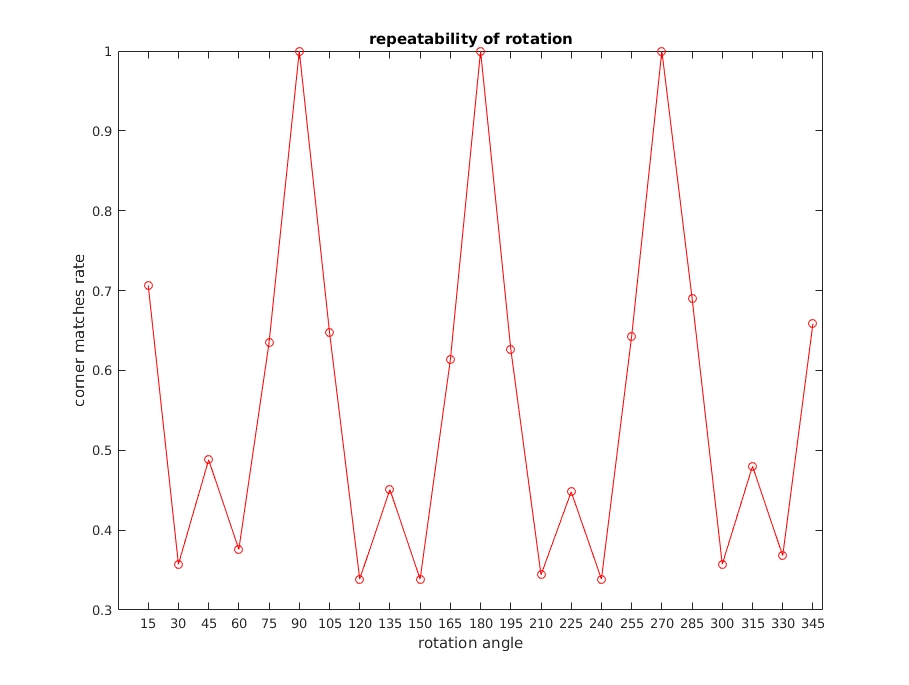
\includegraphics[width=0.8\textwidth]{hw1_fig7.png}
					\caption{图像旋转情况下Harris角点检出率的分布}
				\end{figure}
				\clearpage
				\begin{figure}[htbp!]
					\centering
					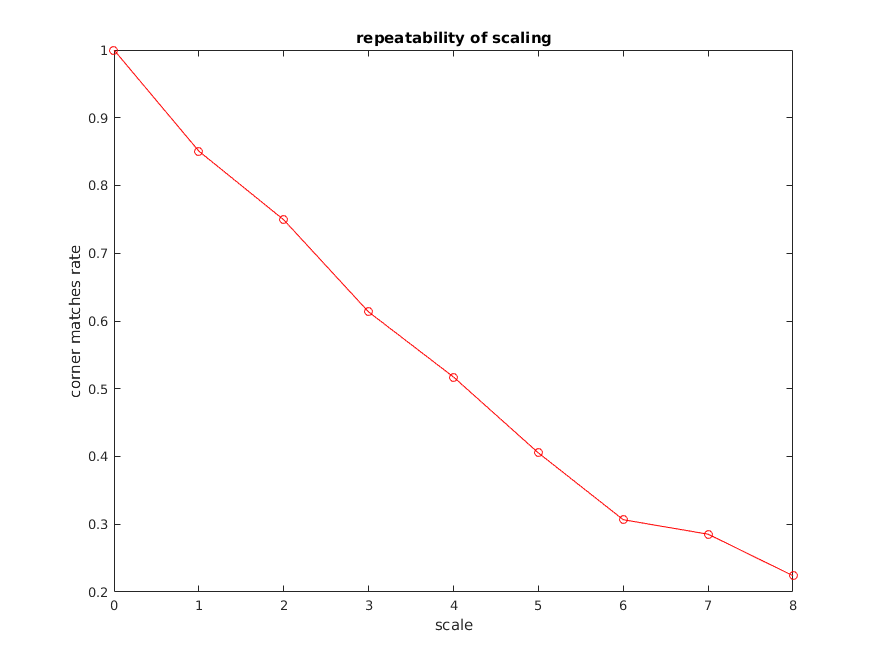
\includegraphics[width=0.8\textwidth]{hw1_fig8.png}
					\caption{图像缩放情况下Harris角点检出率的分布}
				\end{figure}

		\subsection{Robustness of SIFT Keypoints to Rotation and Scaling}
			这里我设置了两个参数,分别为:PEAK\_THRESH= $1$,EDGE\_THRESH= $5$,共检出503个特征。
			\clearpage
			\subsubsection{(a)}
				\begin{figure}[htbp!]
					\centering
					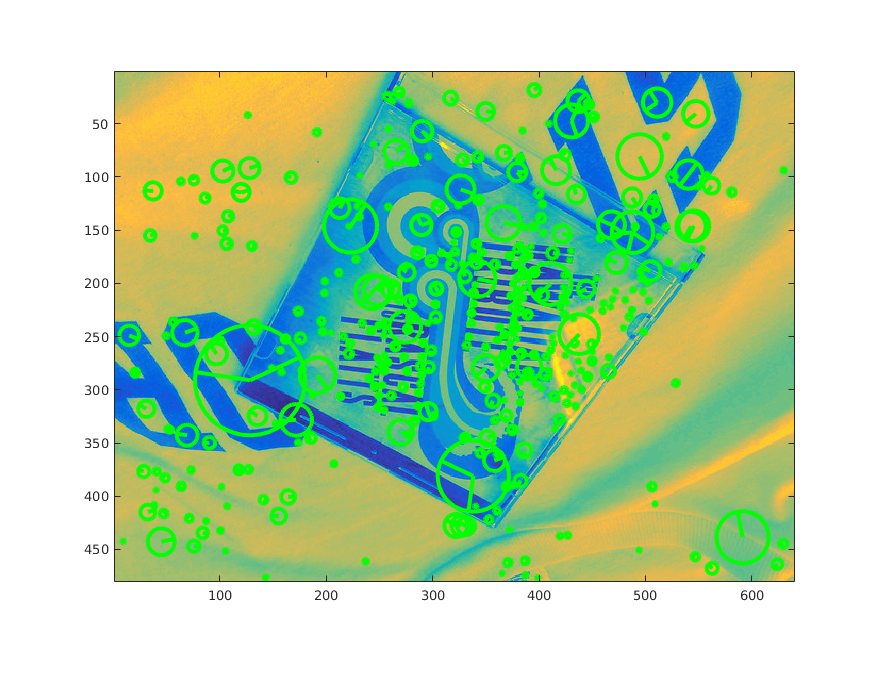
\includegraphics[width=0.8\textwidth]{hw1_fig9.png}
					\caption{SIFT算子检测的结果}
				\end{figure}
				从图中可以看出,SIFT特征主要出现在有显著结构信息的地方,相对于Harris角点来说,SIFT算法检出特征的分布更加广泛。
			\clearpage
			\subsubsection{(b)}
				\begin{figure}[htbp!]
					\centering
					\subfigure[图像旋转情况下SIFT算子检出率的分布]{
					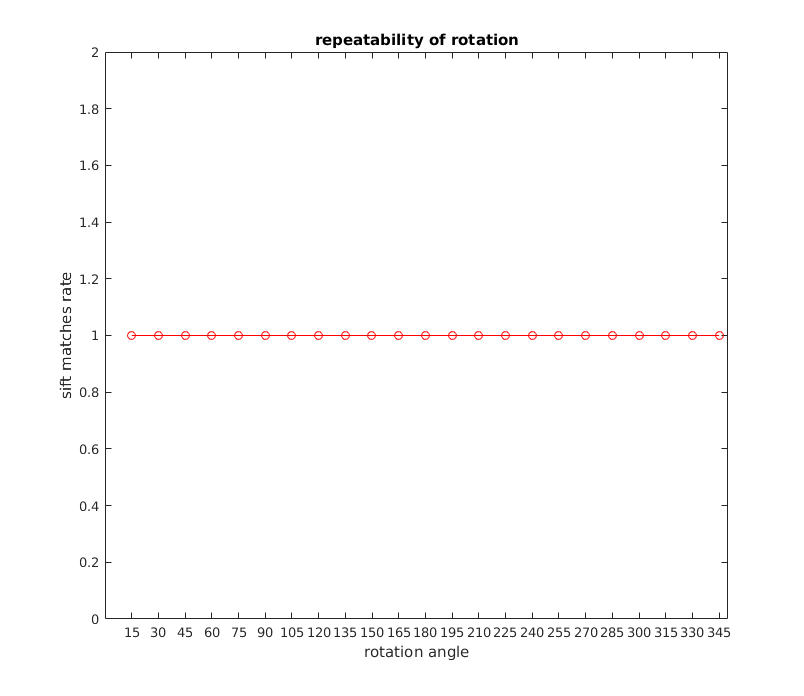
\includegraphics[width=0.4\textwidth]{hw1_fig10.png}}
					\subfigure[图像旋转情况下Harris角点检出率的分布]{
					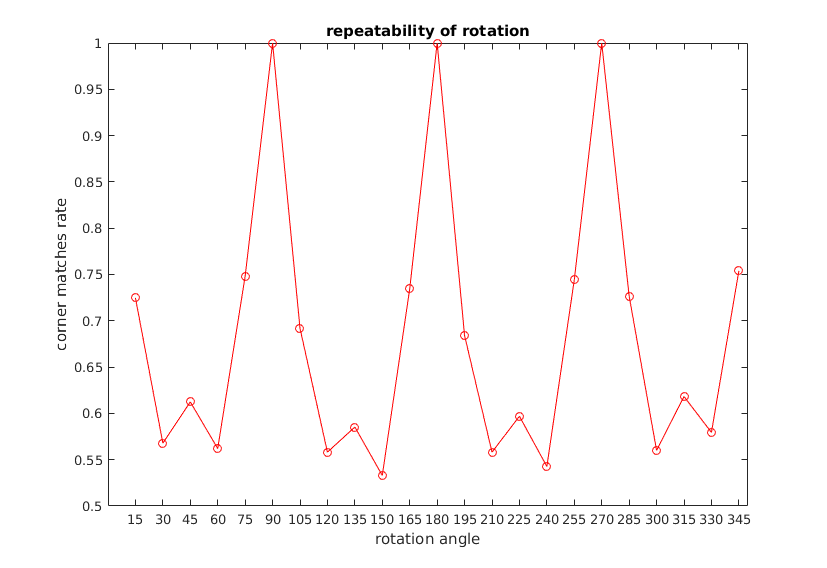
\includegraphics[width=0.4\textwidth]{hw1_fig3.png}}
					\caption{图像旋转情况下两种算法检出率的对比}
				\end{figure}
				从上图可以看出,SIFT算子在旋转情况下依然具有100\%的检出率,因此显然SIFT算子对于旋转具有更好的鲁棒性。
			\subsubsection{(c)}
				\begin{figure}[htbp!]
					\centering
					\subfigure[图像缩放情况下SIFT算子检出率的分布]{
					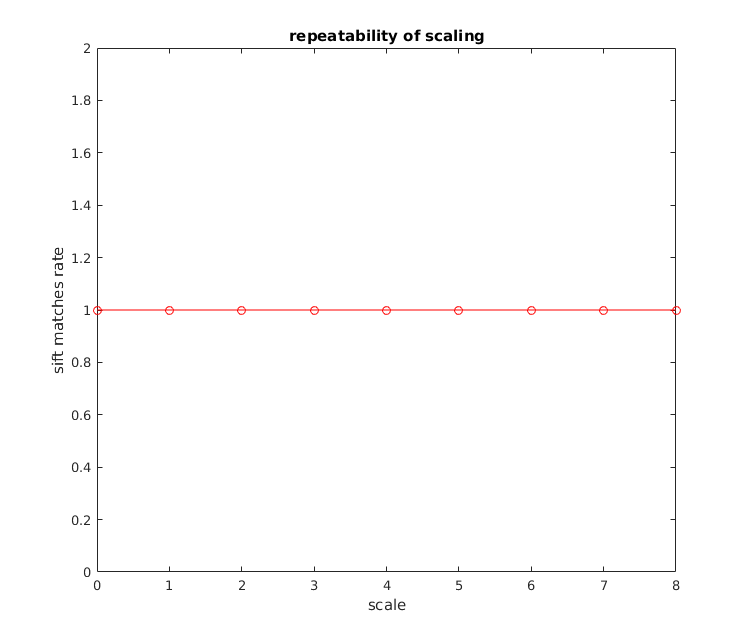
\includegraphics[width=0.4\textwidth]{hw1_fig11.png}}
					\subfigure[图像缩放情况下Harris角点检出率的分布]{
					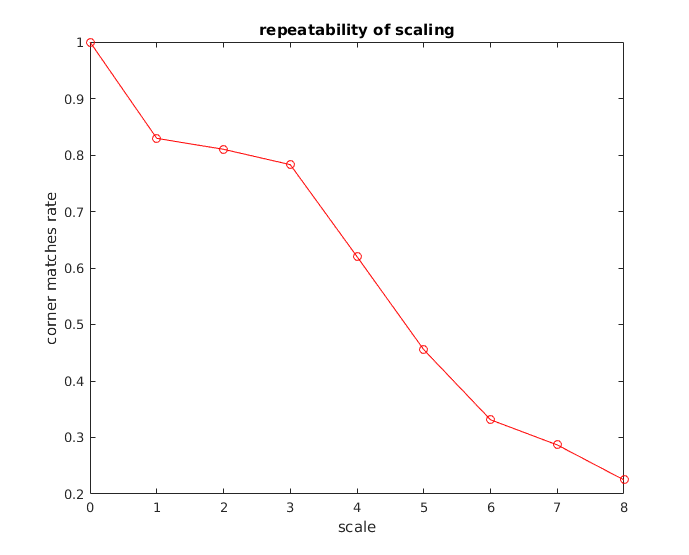
\includegraphics[width=0.4\textwidth]{hw1_fig4.png}}
					\caption{图像缩放情况下两种算法检出率的对比}
				\end{figure}
				从上图可以看出,SIFT算子在缩放情况下依然具有100\%的检出率,因此显然SIFT算子对于缩放具有更好的鲁棒性。
			\clearpage
			\subsubsection{其余数据的数值实验结果}
				\begin{figure}[htbp!]
					\centering
					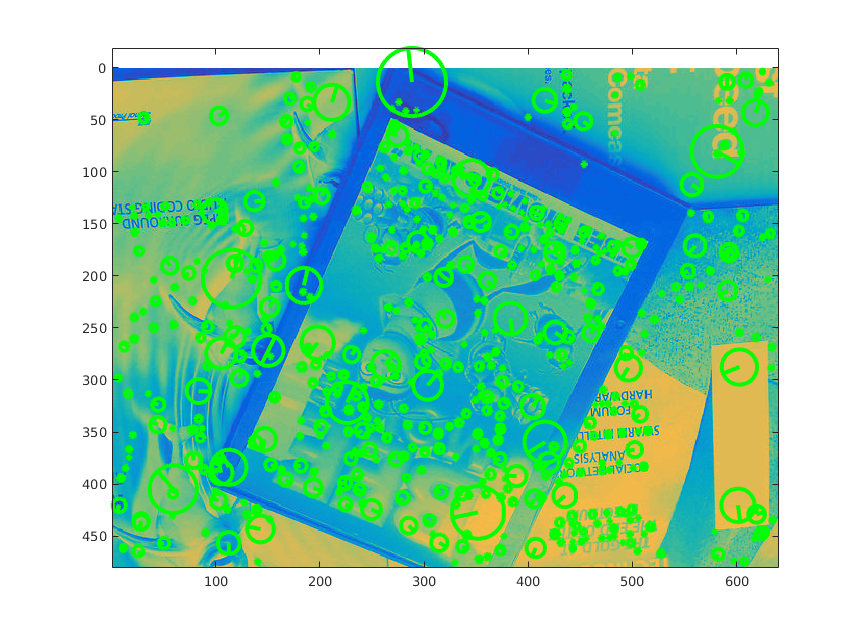
\includegraphics[width=0.8\textwidth]{hw1_fig12.png}
					\caption{SIFT算子检测的结果}
				\end{figure}
				\begin{figure}[htbp!]
					\centering
					\subfigure[图像旋转情况下SIFT算子检出率的分布]{
					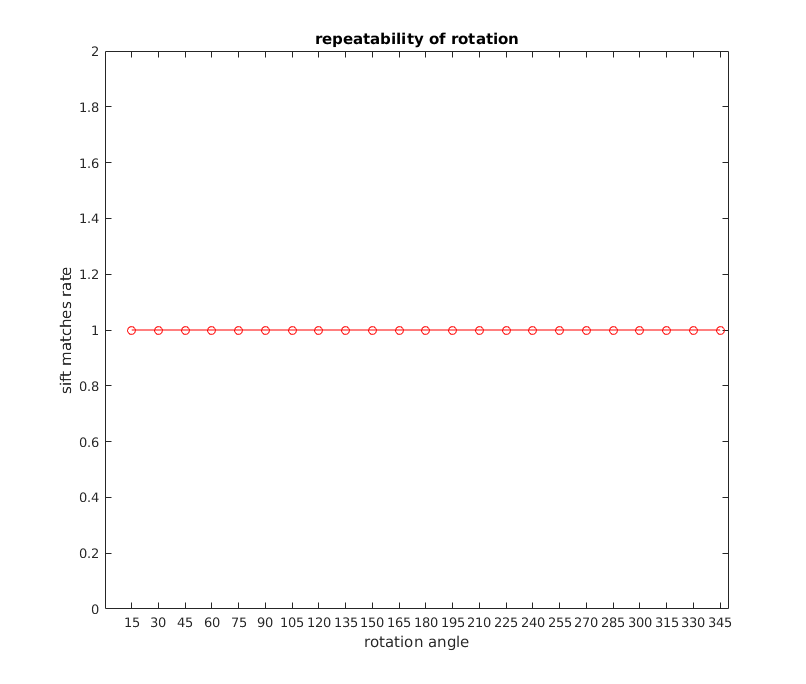
\includegraphics[width=0.4\textwidth]{hw1_fig13.png}}
					\subfigure[图像旋转情况下Harris角点检出率的分布]{
					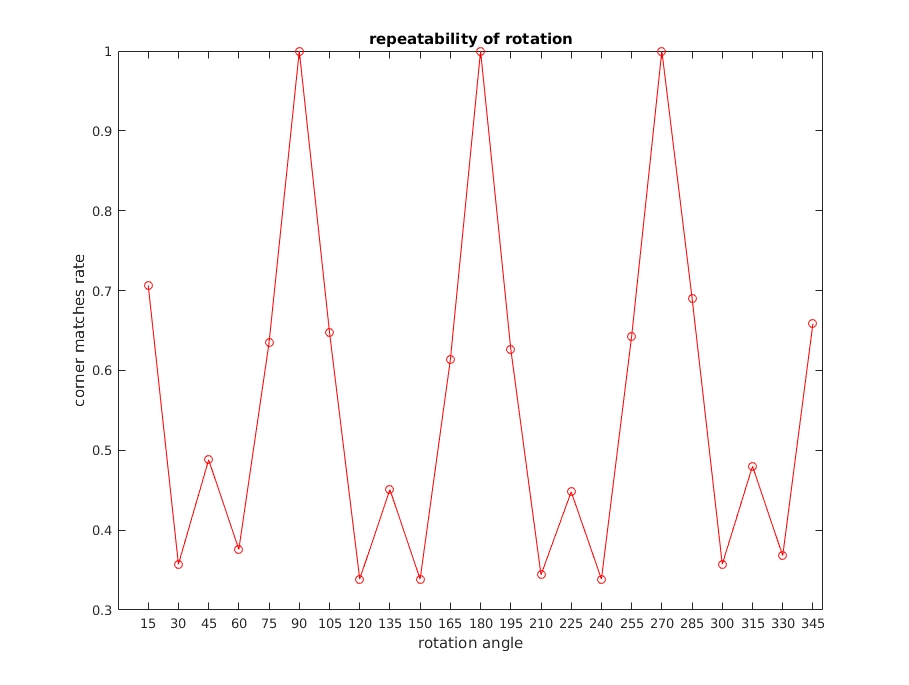
\includegraphics[width=0.4\textwidth]{hw1_fig7.png}}
					\caption{图像旋转情况下两种算法检出率的对比}
				\end{figure}
				\begin{figure}[htbp!]
					\centering
					\subfigure[图像缩放情况下SIFT算子检出率的分布]{
					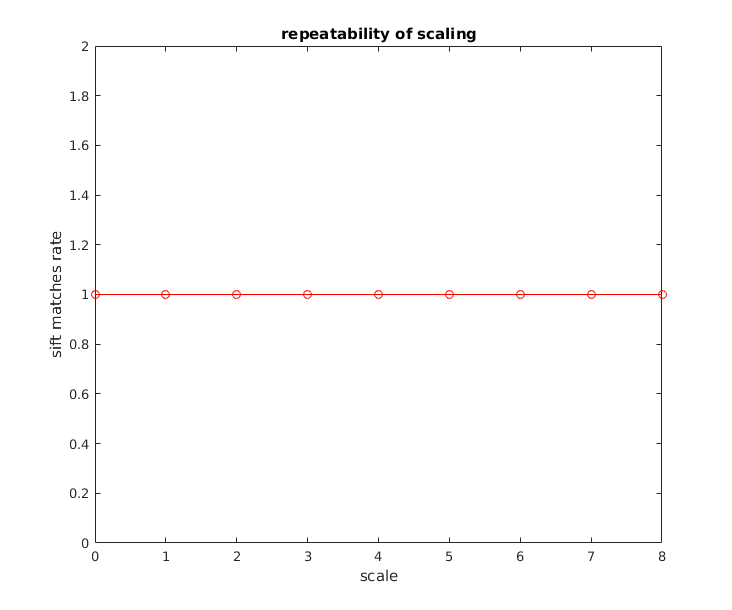
\includegraphics[width=0.4\textwidth]{hw1_fig14.png}}
					\subfigure[图像缩放情况下Harris角点检出率的分布]{
					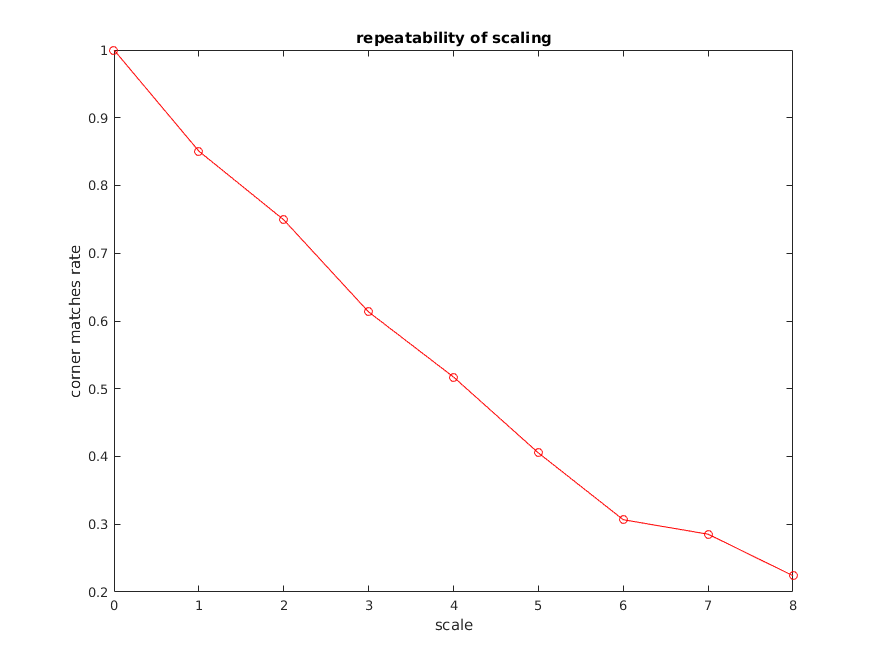
\includegraphics[width=0.4\textwidth]{hw1_fig8.png}}
					\caption{图像缩放情况下两种算法检出率的对比}
				\end{figure}
			\clearpage
		\subsection{Robustness of the SIFT Descriptor}
			\subsubsection{(a)}
				\begin{figure}[htbp!]
					\centering
					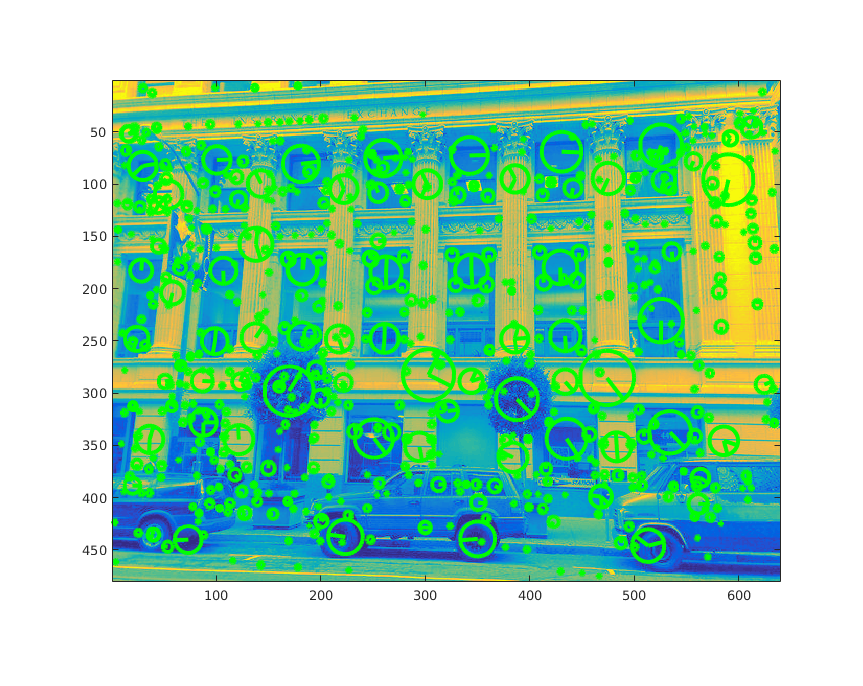
\includegraphics[width=0.8\textwidth]{hw1_fig15.png}
					\caption{SIFT算子检测的结果}
				\end{figure}
			\clearpage
			\subsubsection{(b)}
				\begin{figure}[htbp!]
					\centering
					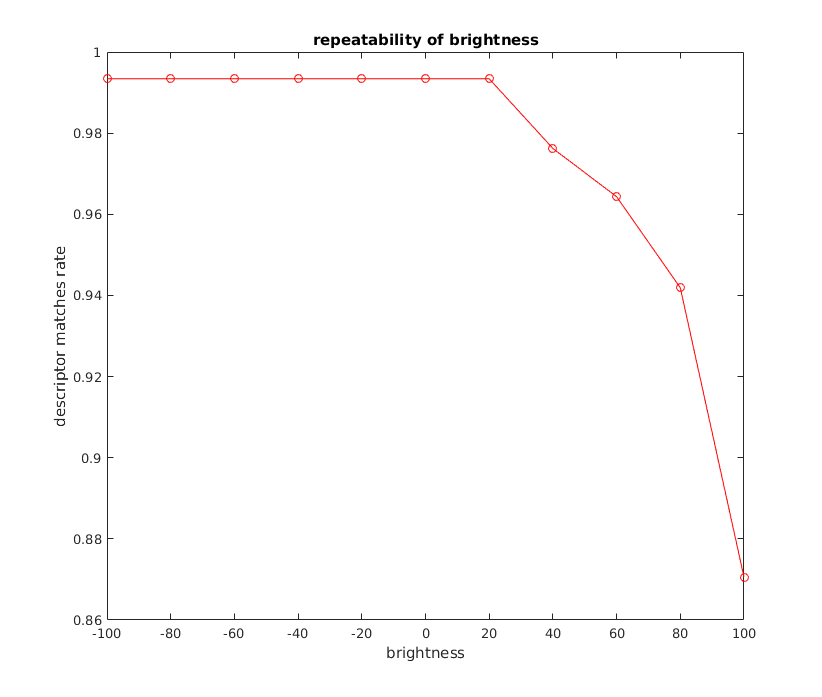
\includegraphics[width=0.8\textwidth]{hw1_fig16.png}
					\caption{SIFT算子随亮度改变的检出率分布}
				\end{figure}
			\clearpage
			\subsubsection{(c)}
				\begin{figure}[htbp!]
					\centering
					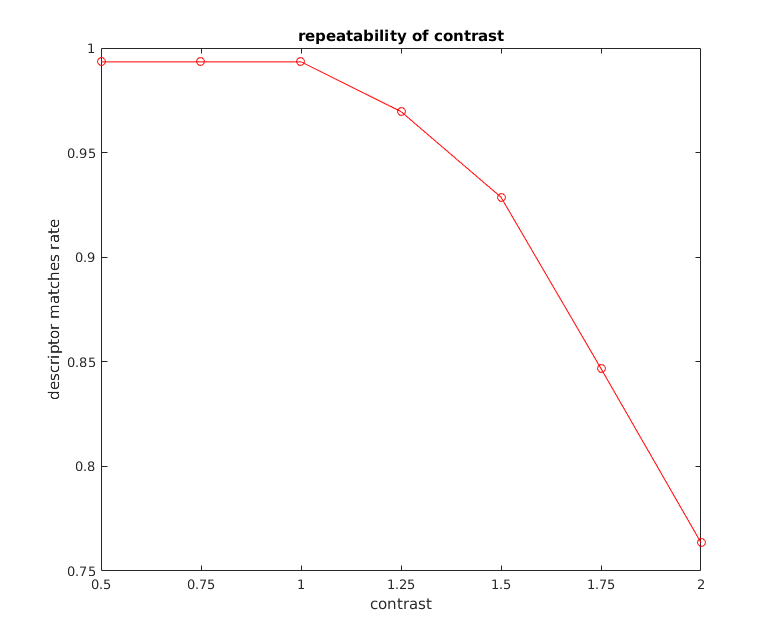
\includegraphics[width=0.8\textwidth]{hw1_fig17.png}
					\caption{SIFT算子随对比度改变的检出率分布}
				\end{figure}
			\clearpage
			\subsubsection{(d)}
				\begin{figure}[htbp!]
					\centering
					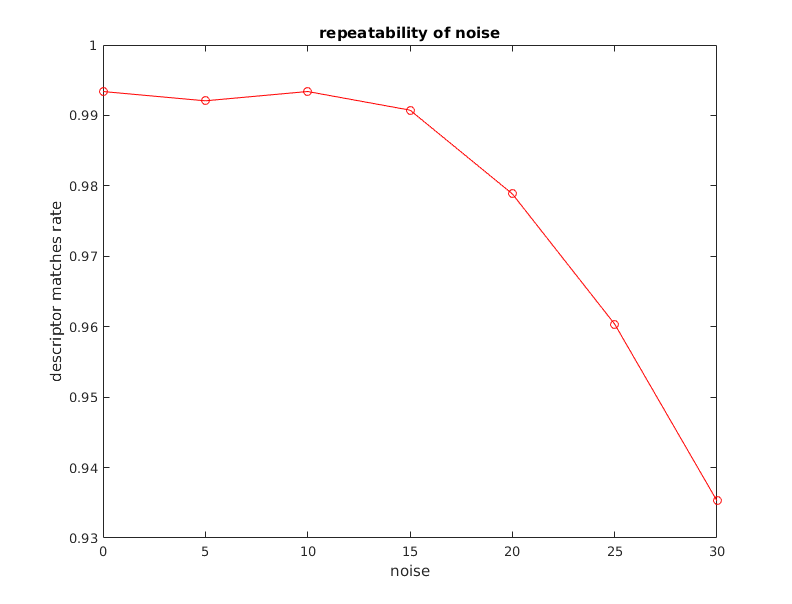
\includegraphics[width=0.8\textwidth]{hw1_fig18.png}
					\caption{SIFT算子随高斯噪声水平改变的检出率分布}
				\end{figure}
			\clearpage
			\subsubsection{(e)}
				\begin{figure}[htbp!]
					\centering
					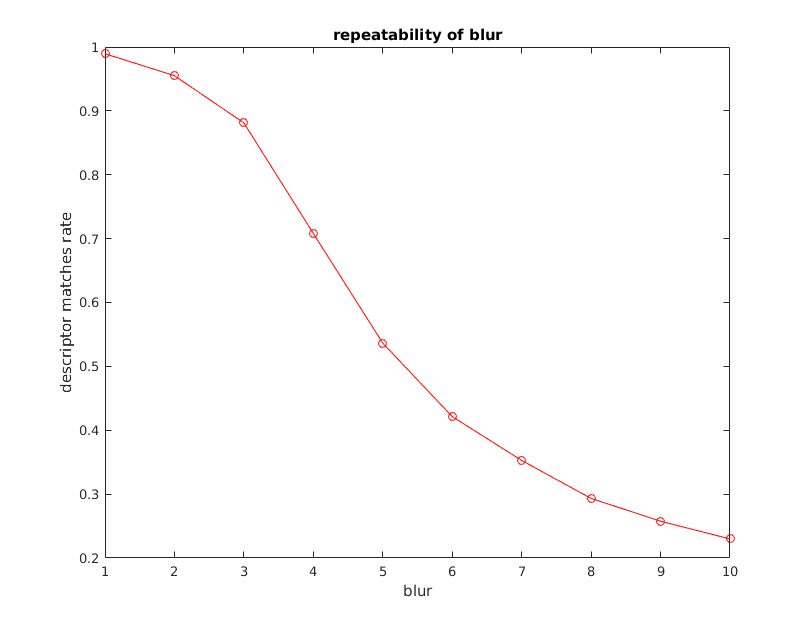
\includegraphics[width=0.8\textwidth]{hw1_fig19.png}
					\caption{SIFT算子随高斯模糊水平改变的检出率分布}
				\end{figure}
		从上面各图可以看出,SIFT算子随亮度,对比度,噪声水平,模糊水平的增加检出率逐渐降低,其中,SIFT算子对亮度,对比度和噪声在小幅度变化的情况下具有较好的鲁棒性,SIFT算子的检出率不会有较大变化,而在大幅度变化的情况下,随着图像细节的逐渐丢失,SIFT算子也不再具有鲁棒性。

  \section{软件版本及测试平台信息}
    这部分内容请参看源代码所在文件夹内的REAME文件。
\end{document}
